
\documentclass[11pt,a4paper]{article}
\usepackage[margin=2cm]{geometry}
\usepackage{graphicx}
\usepackage{booktabs}
\usepackage{array}
\usepackage{multirow}
\usepackage{caption}
\usepackage{float}
\usepackage{newtxtext,newtxmath}
\usepackage{setspace}
\usepackage{titlesec}
\usepackage[hidelinks]{hyperref}
\usepackage{enumitem}

\setstretch{1.05}
\setlength{\parindent}{0pt}
\setlength{\parskip}{0.6em}
\titleformat{\section}{\bfseries\large}{\thesection.}{0.8em}{}
\titleformat{\subsection}{\itshape\normalsize}{\thesubsection}{0.6em}{}
\captionsetup{font=small}

\begin{document}

{\bfseries Twelfth International Conference on Remote Sensing and Geoinformation of the Environment\\
27--29 April, 2026 -- Paphos, Cyprus\par}

\vspace{1.2em}

{\LARGE\bfseries FPGA-accelerated neural network for wildfire pixel classification\par}

\vspace{0.8em}

{\large C. Dionysiou$^{A}$[0009-0008-8865-4549], P. Antoniou$^{A}$, H. E. Michail$^{A}$\par}
{\normalsize $^{A}$Department of Electrical Engineering, Cyprus University of Technology, 30 Archbishop Kyprianou Str., Limassol 3036, Cyprus\par}
{\normalsize E-mail: cs.dionysiou@edu.cut.ac.cy\par}

\section*{Abstract}

Real-time wildfire detection on edge devices requires millisecond-scale inference with low power consumption, yet many image-based fire monitoring systems still depend on graphics processing units (GPUs) or cloud processing, which increase latency, energy use and deployment complexity. This paper presents a field-programmable-gate-array (FPGA) approach for early wildfire indication from RGB imagery using a compact multilayer perceptron (MLP) that performs per-pixel fire/non-fire classification within a streaming pipeline. The proposed workflow covers dataset preparation, pixel-level supervision from segmentation masks, software training in Python, fixed-point quantisation, coefficient export and synthesizable VHDL inference targeting Xilinx FPGA platforms. To make the model hardware-efficient, the arithmetic is implemented in fixed-point form and the sigmoid nonlinearity is realised through a lookup-table (LUT) approximation. The architecture is organised as reusable multiplier and neuron modules integrated in a top-level streaming design that can process continuous RGB input data. Experimental results show that the fixed-point implementation preserves useful predictive performance while maintaining a small hardware footprint. The implemented design reaches approximately 80\% validation accuracy on the main target, achieves an average precision of 0.781 in software evaluation, operates at 74.25 MHz on a Zynq UltraScale+ MPSoC (ZCU106), and sustains 1.782 Gbit/s steady-state throughput with 121.2 ns end-to-end latency. Additional synthesis results on Spartan-7 and Artix-7 devices show that the same VHDL design scales across multiple FPGA families. These results demonstrate that compact neural inference for wildfire monitoring can be executed locally in reconfigurable hardware, supporting low-latency and low-cost fire alert systems for distributed sensing environments.

\textbf{Keywords:} Wildfire detection; FPGA; Artificial neural network; multilayer perceptron; VHDL

\section{Introduction}

Wildfires remain a major environmental and societal threat, and early detection is essential for limiting damage, supporting evacuation decisions and improving the efficiency of emergency response. Image-based methods are attractive because they can provide continuous visual monitoring from satellites, airborne platforms or fixed cameras. Recent remote-sensing literature shows strong progress in wildfire detection and mapping using deep learning, especially when multispectral or hyperspectral information is available (Alsharif et al., 2023; Filizzola et al., 2023). However, the computational cost of many modern vision models makes real-time deployment at the edge difficult, particularly in remote locations where bandwidth, power and communication infrastructure are limited.

For camera-based monitoring, low-complexity fire detection remains important. Classical computer-vision studies demonstrated that flame colour and motion provide useful cues, but also showed that colour-only approaches can produce false alarms in the presence of fire-like objects or strong illumination changes (Celik and Demirel, 2009). This creates a practical design tension: higher-capacity models can improve robustness, but lightweight models are easier to integrate into embedded sensing systems. Field-programmable gate arrays (FPGAs) are well suited to this problem because they offer parallel arithmetic, predictable latency and customisable precision, enabling hardware-efficient inference pipelines close to the sensor (Hamdan, 2017).

This paper presents a hardware-first wildfire pixel classifier based on a compact RGB MLP implemented in fixed-point VHDL. The main contributions are threefold: first, an end-to-end software-to-hardware flow that converts pixel-level wildfire labels into quantised coefficients and a synthesizable inference core; second, a verification path combining software evaluation with image-level RTL simulation; and third, a cross-device implementation study spanning ZCU106, Spartan-7 and Artix-7 targets. Instead of processing image patches or convolutional feature maps, the proposed system classifies each RGB pixel independently, which simplifies the computational graph and maps naturally to multiply-accumulate datapaths in FPGA fabric.

\section{Background and motivation}

Wildfire detection from imagery spans a wide range of sensing modalities and algorithms. Satellite and hyperspectral approaches can exploit rich spectral information and large-area coverage, often achieving high detection or mapping quality, but they typically require heavier preprocessing and more demanding models (Alsharif et al., 2023; Filizzola et al., 2023). In contrast, fixed camera systems offer simpler data acquisition and continuous local monitoring, which makes them attractive for near-sensor detection in remote deployments. For this type of application, the cost of inference becomes as important as predictive accuracy.

MLPs are a reasonable baseline for per-pixel classification because they learn a nonlinear decision boundary in RGB space while retaining a simple feed-forward structure. Earlier FPGA studies showed that MLP-style networks can be implemented directly in VHDL and mapped to hardware as multipliers, accumulators and activation blocks (Himavathi, Anitha and Muthuramalingam, 2007). The same literature also shows that an inference-only deployment flow is practical: the model is trained offline in software, then weights and biases are exported to a fixed hardware datapath (Himavathi, Anitha and Muthuramalingam, 2007; Hamdan, 2017).

A second important design choice concerns numeric representation. Floating-point arithmetic is expensive on FPGA devices, whereas fixed-point arithmetic reduces logic cost and can improve timing closure, parallelism and overall efficiency (Hamdan, 2017; Kara et al., 2017). Nonlinear functions such as sigmoid are also expensive to compute directly in RTL, so lookup-table approximations are commonly used in hardware neural-network designs (Himavathi, Anitha and Muthuramalingam, 2007). The present work therefore combines a compact MLP, fixed-point arithmetic and LUT-based activation to produce a deterministic and resource-conscious wildfire classification core.

\section{Methodology}

\subsection{Dataset preparation and software flow}

The dataset is organised as wildfire and non-fire RGB images accompanied by segmentation masks. These masks are used to derive pixel-level labels, allowing the problem to be formulated as binary classification with three inputs per sample: red, green and blue intensity values. Each pixel is treated as an independent training example, which keeps the feature vector small and aligns the software model with the intended FPGA streaming architecture. During data preparation, pixel values are normalised and the sampling procedure is structured to reduce class imbalance between fire and non-fire observations.

The neural network is trained offline in Python as a compact 3-7-2 MLP. The fixed-point export keeps the input representation in 8-bit RGB, stores quantised weights and biases as signed integers, and realises the sigmoid using a 12-bit address and 8-bit output LUT. In total, the network is represented by 44 fixed-point parameters, which keeps the hardware footprint small enough for direct FPGA integration. After training, the learned weights and biases are exported as fixed-point coefficients. An additional script generates a sigmoid lookup table over a bounded input range so that the hardware implementation can reproduce the nonlinear activation without resorting to floating-point operations. This workflow follows the established pattern of software training followed by fixed-coefficient hardware inference and reflects common FPGA design trade-offs between precision, cost and numerical fidelity (Himavathi, Anitha and Muthuramalingam, 2007; Kara et al., 2017; Hamdan, 2017).

\subsection{Fixed-point export and verification flow}

The complete co-design flow contains six stages: dataset preparation, software training, evaluation of the floating-point network, fixed-point quantisation, LUT generation and VHDL verification. Exported vectors are used later in simulation so that the RTL design can be checked. This separation between model quality evaluation and implementation verification is important in FPGA machine-learning workflows because it isolates quantisation loss from RTL errors and provides traceable equivalence between the software model and the final hardware datapath (Hamdan, 2017).

\section{FPGA implementation}

The FPGA implementation is written in VHDL and organised as a modular streaming architecture. A global configuration package defines the fixed-point widths and scaling parameters used across the datapath. The core arithmetic is realised through multiplier modules and neuron modules that perform weighted sums, bias addition and activation interfacing. At the top level, the \texttt{nn\_rgb} entity connects the network layers and coordinates the movement of valid pixel data through the pipeline.

To reduce hardware cost, the design uses fixed-point multiply-accumulate operations and evaluates the sigmoid through a dedicated LUT block stored in on-chip memory. This replaces expensive exponential arithmetic with a deterministic memory access. Such LUT-based activation is common in FPGA neural-network implementations because it offers a predictable timing profile and a favourable trade-off between memory usage and numerical fidelity (Himavathi, Anitha and Muthuramalingam, 2007; Su et al., 2023). The resulting inference core is synthesizable in Vivado and targets multiple Xilinx families, while remaining largely vendor-neutral apart from the sigmoid read-only-memory (ROM) wrapper.

Verification is performed in simulation by replaying software-generated test vectors and comparing the RTL outputs with test probabilities. This process validates both the arithmetic datapath and the alignment of streaming control signals, which is essential in deterministic pixel-stream pipelines. After functional verification, the design is synthesised and implemented in Vivado, where timing, resource utilisation and throughput are measured to evaluate the practical feasibility of the proposed wildfire classifier.

\section{Results and discussion}

\subsection{Software evaluation}

Figure~\ref{fig:software} summarises the main software-side validation results. The confusion matrix shows that, at the chosen operating threshold, the model strongly favours detecting the fire class, which yields a large number of correctly detected fire pixels but also a sizeable false-positive count on non-fire pixels. This behaviour is consistent with the known limitations of RGB-only fire classifiers, where fire-coloured regions and bright scene structures may be confused with flame pixels.

The precision-recall curve nevertheless shows useful class separability, with an average precision of 0.781 on the validation set. This is an encouraging result for such a small network, especially given that the model uses only per-pixel RGB information.

\begin{figure}[H]
\centering
\begin{minipage}[t]{0.46\linewidth}
\centering
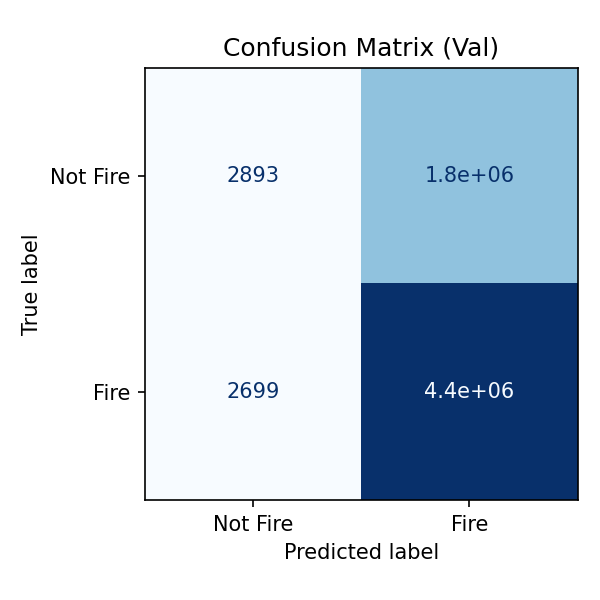
\includegraphics[width=\linewidth]{confusion_matrix.png}
\end{minipage}\hfill
\begin{minipage}[t]{0.46\linewidth}
\centering
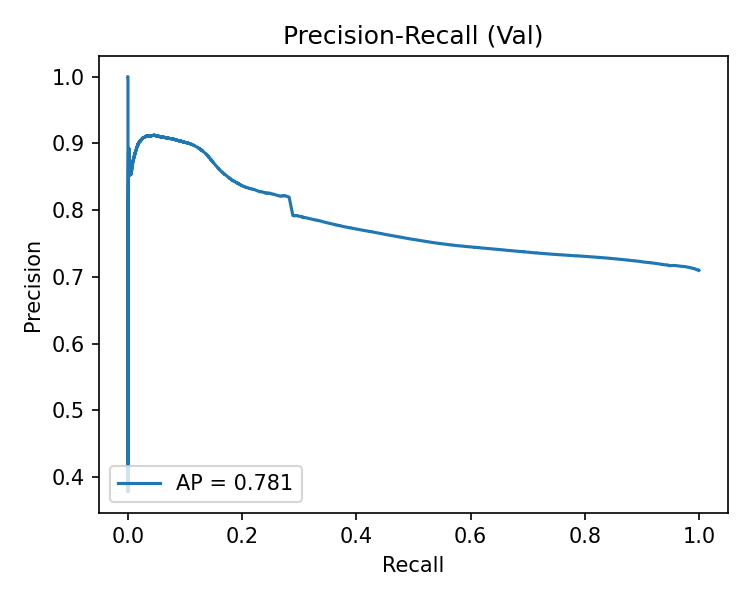
\includegraphics[width=\linewidth]{pr_curve.png}
\end{minipage}
\caption{Software validation results for the wildfire pixel classifier. Left: validation confusion matrix. Right: precision-recall curve with average precision (AP) of 0.781.}
\label{fig:software}
\end{figure}

\subsection{RTL simulation and main hardware target}

Figure~\ref{fig:rtl} shows a qualitative RTL simulation example from the ModelSim/Questa validation flow. The testbench reads a stimulus image, processes it through the VHDL network, and writes an \texttt{image\_response.ppm} output. The left panel shows the thresholded response image, while the right panel overlays the detected regions on the original scene. This example confirms that the streaming datapath is functionally correct at image level and that the output stays aligned with the incoming pixel stream after pipeline delays.

\begin{figure}[H]
\centering
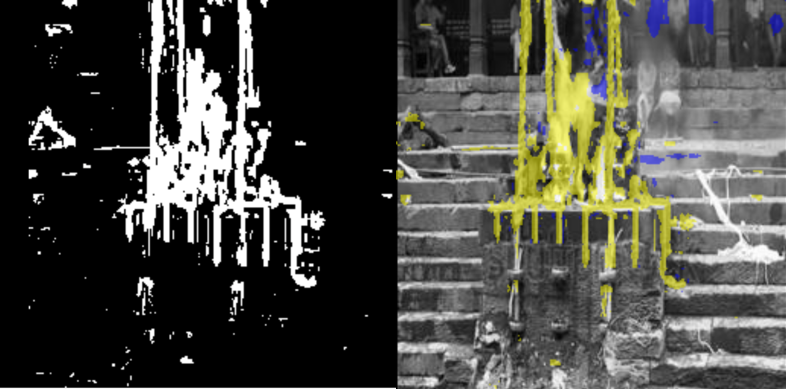
\includegraphics[width=0.88\linewidth]{simulation_output.PNG}
\caption{Example RTL simulation output generated from the image-based testbench. Left: thresholded response image. Right: detection response overlaid on the source frame.}
\label{fig:rtl}
\end{figure}

Table~\ref{tab:zcu} reports the detailed post-implementation results for the ZCU106 target. Post-implementation timing shows a positive worst negative slack, indicating successful timing closure at 74.25 MHz. With a 24-bit RGB input and a nine-cycle end-to-end pipeline delay, the measured latency is 121.2 ns. Because the design is pipelined, it accepts one pixel per clock after the initial fill stage, yielding a steady-state throughput of 1.782 Gbit/s, equivalent to 74.25 Mpixel/s. The hardware cost remains moderate for an FPGA-based neural inference block, using approximately 4850 LUTs, 476 flip-flops and 71 DSP blocks.

\begin{table}[H]
\centering
\caption{Post-implementation summary on the ZCU106 target.}
\label{tab:zcu}
\begin{tabular}{>{\raggedright\arraybackslash}p{0.56\linewidth} >{\centering\arraybackslash}p{0.26\linewidth}}
\toprule
\textbf{Metric} & \textbf{Value} \\
\midrule
Approximate validation accuracy & 79.7\% \\
Worst negative slack (WNS) & 0.077 ns \\
Clock frequency & 74.25 MHz \\
End-to-end latency & 121.2 ns \\
Steady-state throughput & 1.782 Gbit/s \\
Post-implementation LUTs & 4850 \\
Post-implementation FFs & 476 \\
Post-implementation DSPs & 71 \\
\bottomrule
\end{tabular}
\end{table}

\subsection{Cross-device portability}

To assess portability across FPGA families, the same VHDL design was also synthesised for Spartan-7 and Artix-7 devices. The results in Table~\ref{tab:devices} show that the design preserves a very similar area footprint across the three targets while achieving higher maximum frequency on the two 7-series devices. The Artix-7 configuration reaches the highest reported frequency at 94 MHz and also achieves the best throughput-to-area ratio, whereas the Spartan-7 result remains close behind at 90 MHz. These results indicate that the proposed classifier is not tied to a single board and can be retargeted to smaller or lower-cost Xilinx families with only modest changes in performance. In the context of FPGA neural-network implementations, this kind of portability is valuable because hardware comparisons are often strongly shaped by device family and tool flow rather than by network structure alone (Su et al., 2023).

\begin{table}[H]
\centering
\caption{Cross-device implementation comparison.}
\label{tab:devices}
\begin{tabular}{lcccccc}
\toprule
\textbf{Board} & \textbf{f (MHz)} & \textbf{Area (LUT)} & \textbf{Throughput} & \textbf{Thr./area} & \textbf{CLB} & \textbf{Slice} \\
 &  &  & \textbf{(Gbps)} & \textbf{(Gbps/kLUT)} &  &  \\
\midrule
ZCU106 & 74.25 & 4850 & 1.782 & 0.367 & 809 & 809 \\
Spartan-7 & 90.00 & 5060 & 2.184 & 0.432 & 784 & 1568 \\
Artix-7 & 94.00 & 5085 & 2.256 & 0.444 & 791 & 1582 \\
\bottomrule
\end{tabular}
\end{table}

The main strength of the approach is therefore not maximum representational power, but deployability. Unlike larger CNN-based models, the RGB-only MLP can be mapped to a deterministic datapath with low latency and no dependency on external computing infrastructure. The main limitation is that the classifier does not exploit spatial or temporal context. As reported in prior fire-detection literature, colour-driven models can struggle with reflective surfaces, bright light sources or fire-like objects (Celik and Demirel, 2009). Nevertheless, the presented design establishes a practical baseline for hardware wildfire monitoring and a foundation for more advanced future architectures.

\section{Conclusion and Future Work}

This paper presented an FPGA-based wildfire pixel classifier built around a compact RGB multilayer perceptron. The proposed methodology links software training and hardware deployment through fixed-point quantisation, coefficient export, LUT generation, VHDL implementation and simulation-based verification. The software results show useful ranking ability, the RTL flow produces correct image-level responses, and the implemented design scales across ZCU106, Spartan-7 and Artix-7 with consistent area and real-time throughput. Within the scope of this work, the emphasis is therefore on deterministic low-latency deployment rather than maximum model complexity.

Future work will focus on extending the current design with richer input information and stronger context modelling. Possible next steps include adding temporal cues for video-based fire dynamics, incorporating spatial features or lightweight convolutional stages, and evaluating multispectral inputs when available. Another important direction is to study partial on-device adaptation, including hardware support for gradient-based update mechanisms, while preserving the deterministic timing advantages demonstrated by the current inference core.

\section*{References}

Alsharif, M.A. et al. (2023) `Deep learning approaches for wildland fires using satellite remote sensing data: detection, mapping, and prediction', \textit{Fire}, 6(5), p.~192. Available at: \url{https://www.mdpi.com/2571-6255/6/5/192}.

Celik, T. and Demirel, H. (2009) `Computer vision based method for real-time fire and flame detection', \textit{Expert Systems with Applications}, 36(2), pp.~1760--1765. Available at: \url{https://research.itu.edu.tr/en/publications/computer-vision-based-method-for-real-time-fire-and-flame-detecti/}.

Filizzola, A. et al. (2023) `Wildfire detection using convolutional neural networks and PRISMA hyperspectral imagery: A spatial-spectral analysis', \textit{Remote Sensing}, 15(19), p.~4855. Available at: \url{https://www.mdpi.com/2072-4292/15/19/4855}.

Hamdan, M.H. (2017) \textit{FPGA architecture for deep learning and its application to planetary robotics}. Iowa State University. Available at: \url{https://lib.dr.iastate.edu/etd/15874/}.

Himavathi, S., Anitha, D. and Muthuramalingam, A. (2007) `FPGA implementation of a multilayer perceptron neural network using VHDL'. Available at: \url{https://ieeexplore.ieee.org/document/770860}.

Kara, K., Alistarh, D., Alonso, G., Mutlu, O. and Zhang, C. (2017) `FPGA-accelerated dense linear machine learning: A precision-convergence trade-off', in \textit{2017 IEEE 25th Annual International Symposium on Field-Programmable Custom Computing Machines (FCCM)}.

Su, Y., Seng, K.P., Ang, L.M. and Smith, J. (2023) `Binary neural networks in FPGAs: Architectures, tool flows and hardware comparisons', \textit{Sensors}, 23(22), 9254. Available at: \url{https://www.mdpi.com/1424-8220/23/22/9254}.

\end{document}
